% This file was created by tikzplotlib v0.9.8.
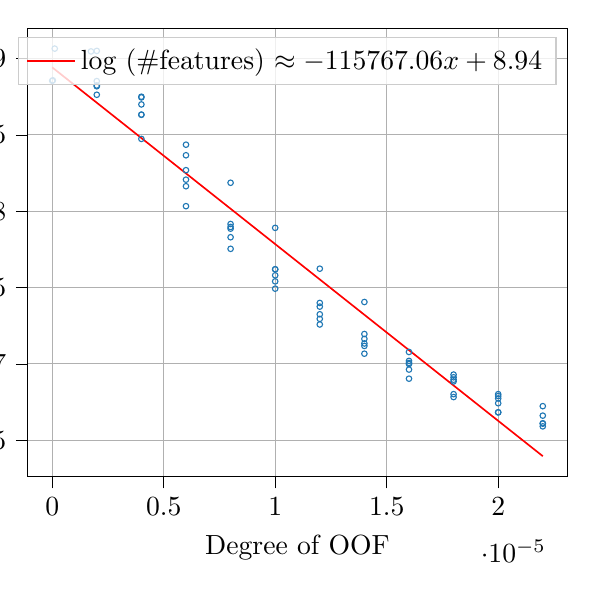
\begin{tikzpicture}[trim axis left,trim axis right]

\definecolor{color0}{rgb}{0.12156862745098,0.466666666666667,0.705882352941177}

\begin{axis}[
legend cell align={left},
legend style={fill opacity=0.8, draw opacity=1, text opacity=1, draw=white!80!black},
tick align=outside,
tick pos=left,
% title={Log feature count vs. OOF},
x grid style={white!69.0196078431373!black},
xlabel={Degree of OOF},
xmin=-1.09892007559144e-06, xmax=2.31000189170211e-05,
xtick style={color=black},
y grid style={white!69.0196078431373!black},
ylabel={log (\#features)},
xmajorgrids,
ymajorgrids,
ymin=6.26154869922026, ymax=9.1982215266363,
ytick style={color=black}
]
\addplot [draw=color0, fill=color0, forget plot, mark=*, mark size=1, only marks, mark options={solid,fill opacity=0}]
table{%
x  y
2.89713740402389e-08 8.85694575615902
1.79997717738205e-05 6.88448665204278
9.99997577071001e-06 7.54009032014532
2.00011560321043e-06 8.8180382503943
6.00014606118044e-06 8.43533216493592
1.20001917481398e-05 7.6231530684769
2.19998022317905e-05 6.61069604471776
1.99991485475958e-06 8.82335348511379
3.99993008374979e-06 8.63159273172473
5.99994531274e-06 8.20631072579402
1.80000366866596e-05 6.80128303447162
2.00000519156498e-05 6.68210859744981
8.00016129016978e-06 8.18590748148232
1.000017651916e-05 7.89058253465654
1.400020697713e-05 7.40488757561612
1.99997870028003e-05 6.77308037565554
7.99996054173021e-06 7.82923253754359
1.40000062286896e-05 7.11720550316434
1.60002222061202e-05 7.07749805356923
1.19999909997002e-05 7.25770767716004
1.60000214576702e-05 6.96224346426621
4.00013083219977e-06 8.63230599851674
2.20000671446296e-05 6.59030104819669
1.400020697713e-05 7.06646697013696
3.99993008374979e-06 8.74957394808293
7.99996054173021e-06 7.89655270164304
9.99997577071001e-06 7.61923341622681
1.03169680003984e-09 8.85366542803745
1.000017651916e-05 7.49220304261874
2.19998022317905e-05 6.60800062529609
1.99991485475958e-06 8.85180655855245
5.99994531274e-06 8.36613771649628
1.40000062286896e-05 7.16317239084664
1.80000366866596e-05 6.89568269774787
2.00011560321043e-06 8.76233304060234
4.00013083219977e-06 8.47324130388705
6.00014606118044e-06 8.03268487596762
8.00016129016978e-06 7.75319426988434
1.20001917481398e-05 7.29437729928882
1.60002222061202e-05 6.90274273715859
1.79997717738205e-05 6.78219205600679
1.19999909997002e-05 7.37462901521894
1.60000214576702e-05 7.0057890192535
2.00000519156498e-05 6.74170069465205
2.20000671446296e-05 6.66057514983969
1.99997870028003e-05 6.68210859744981
1.14187389609749e-07 9.06473639811739
1.74120792746993e-06 9.04629085996968
4.00013083219977e-06 8.69901462316851
2.19998022317905e-05 6.72262979485545
1.99991485475958e-06 9.04970202601337
3.99993008374979e-06 8.74512525946224
9.99997577071001e-06 7.61923341622681
1.80000366866596e-05 6.91174730025167
6.00014606118044e-06 8.16337131645991
8.00016129016978e-06 7.88532923927319
1.20001917481398e-05 7.32448997934853
1.60002222061202e-05 6.9985096422506
7.99996054173021e-06 7.91571319938212
2.00000519156498e-05 6.78897174299217
1.000017651916e-05 7.57967882309046
1.79997717738205e-05 6.92951677076365
1.99997870028003e-05 6.80128303447162
1.19999909997002e-05 7.39878627541995
1.40000062286896e-05 7.19518732017871
1.60000214576702e-05 7.01929665371504
1.400020697713e-05 7.13329595489607
5.99994531274e-06 8.2684753889826
};
\addplot [semithick, red]
table {%
1.03169680003984e-09 8.94179754399353
2.89713740402389e-08 8.93856304962636
1.14187389609749e-07 8.92869784180801
1.74120792746993e-06 8.74034245317065
1.99991485475958e-06 8.71039271209553
1.99991485475958e-06 8.71039271209553
1.99991485475958e-06 8.71039271209553
2.00011560321043e-06 8.71036947203703
2.00011560321043e-06 8.71036947203703
3.99993008374979e-06 8.47885682365952
3.99993008374979e-06 8.47885682365952
3.99993008374979e-06 8.47885682365952
4.00013083219977e-06 8.47883358360112
4.00013083219977e-06 8.47883358360112
4.00013083219977e-06 8.47883358360112
5.99994531274e-06 8.24732093522351
5.99994531274e-06 8.24732093522351
5.99994531274e-06 8.24732093522351
6.00014606118044e-06 8.24729769516622
6.00014606118044e-06 8.24729769516622
6.00014606118044e-06 8.24729769516622
7.99996054173021e-06 8.01578504678751
7.99996054173021e-06 8.01578504678751
7.99996054173021e-06 8.01578504678751
8.00016129016978e-06 8.01576180673031
8.00016129016978e-06 8.01576180673031
8.00016129016978e-06 8.01576180673031
9.99997577071001e-06 7.7842491583527
9.99997577071001e-06 7.7842491583527
9.99997577071001e-06 7.7842491583527
1.000017651916e-05 7.78422591829431
1.000017651916e-05 7.78422591829431
1.000017651916e-05 7.78422591829431
1.19999909997002e-05 7.5527132699167
1.19999909997002e-05 7.5527132699167
1.19999909997002e-05 7.5527132699167
1.20001917481398e-05 7.5526900298595
1.20001917481398e-05 7.5526900298595
1.20001917481398e-05 7.5526900298595
1.40000062286896e-05 7.32117738148079
1.40000062286896e-05 7.32117738148079
1.40000062286896e-05 7.32117738148079
1.400020697713e-05 7.3211541414235
1.400020697713e-05 7.3211541414235
1.400020697713e-05 7.3211541414235
1.60000214576702e-05 7.08964149304589
1.60000214576702e-05 7.08964149304589
1.60000214576702e-05 7.08964149304589
1.60002222061202e-05 7.08961825298749
1.60002222061202e-05 7.08961825298749
1.60002222061202e-05 7.08961825298749
1.79997717738205e-05 6.85813627279123
1.79997717738205e-05 6.85813627279123
1.79997717738205e-05 6.85813627279123
1.80000366866596e-05 6.85810560460998
1.80000366866596e-05 6.85810560460998
1.80000366866596e-05 6.85810560460998
1.99997870028003e-05 6.62660038435643
1.99997870028003e-05 6.62660038435643
1.99997870028003e-05 6.62660038435643
2.00000519156498e-05 6.62656971617397
2.00000519156498e-05 6.62656971617397
2.00000519156498e-05 6.62656971617397
2.19998022317905e-05 6.39506449592042
2.19998022317905e-05 6.39506449592042
2.19998022317905e-05 6.39506449592042
2.20000671446296e-05 6.39503382773917
2.20000671446296e-05 6.39503382773917
};
\addlegendentry{log (\#features) $\approx -115767.06x + 8.94$}
\end{axis}

\end{tikzpicture}
